% Provenance (never printed): old terminale S material on the Earth's internal
% heat (geothermal gradient and heat flow, radioactive heat production,
% conduction and convection, mantle convection, geothermal energy). Owner
% (Sync 0/1): heat flow, radiogenic heat production, secular cooling, thermal
% and mantle convection (recall the convection cell of Book 1 g8 first),
% geothermal energy. Geotherm and geothermal gradient are g11.03's; radioactivity,
% half-life, decay law and thermal conductivity are physics' (thermal
% conductivity used as "the rock's thermal conductivity k", never defined);
% hotspot track and plume g11.04's. Figures: figdata/grade-12/internal_heat.py.
\chapter{The Earth's Internal Heat}\label{ch:g12:internal-heat}

Between 1987 and 1995, near the village of Windischeschenbach in Bavaria,
geologists drilled a hole \qty{9101}{m} deep into the \omterm{def:g12:continental-crust:continental-crust}{continental crust}. At the
bottom the rock was at about \qty{265}{\celsius}, too hot to drill any
deeper.
% ledger: gfz:ktb, gfz:ktb30

From about \qty{10}{\celsius} at the surface to \qty{265}{\celsius} at
\qty{9.1}{km} is a rise of about \qty{28}{\celsius} per kilometre, a typical
value. Everywhere on Earth, it gets hotter downwards, so heat flows out of
the Earth all the time. This chapter measures that flow, asks where the heat
comes from, and shows how it moves.
% values: ktb_gradient 28.0 (internal_heat.py, surface temperature taken as 10 degC); ledger: gfz:ktb (gradient about 28 K/km)

\begin{recall}
The \omterm{def:g11:lithosphere-asthenosphere:geotherm}{geotherm} is the curve of temperature against depth beneath a place, and
the \omterm{def:g11:lithosphere-asthenosphere:geotherm}{geothermal gradient} the rise of temperature per kilometre; boreholes
measure 25 to \qty{30}{\celsius} per kilometre near the surface
(\cref{ch:g11:lithosphere-asthenosphere}). Some atoms are radioactive: they
decay at random, the number left falling by half every half-life, and each
decay releases energy, which ends up as heat (the physics books). A
convection cell is a loop of fluid warmed from below, which rises, spreads,
cools and sinks (Book 1, grade 8). At a hotspot, a plate moves over a plume
of hot mantle (\cref{ch:g11:plate-motions}).
\end{recall}
% ledger: usgs:gradient-29 (Book 1 row)

\section{Gradient and heat flow}

\begin{definition}[Heat flow]\label{def:g12:internal-heat:heat-flow}
The \emph{heat flow}\index{heat flow} (or heat flux) at a place is the
power that leaves the Earth's interior through each square metre of its
surface there. It is measured in milliwatts per square metre
(\unit{mW/m^2}).
\end{definition}
% ledger: b2dd10:continents

Heat flows from hot to cold, and the steeper the temperature gradient, the
faster it flows. How much flows also depends on the rock: each rock has a
thermal conductivity $k$, in watts per metre per kelvin, which the physics
books define.

\begin{proposition}[Heat flow and gradient]\label{prop:g12:internal-heat:fourier}
Through rock of thermal conductivity $k$ in which the temperature rises with
depth by a gradient $G$ (in kelvins per metre), the \omterm{def:g12:internal-heat:heat-flow}{heat flow} up towards the
surface is
\[
  q = k\,G .
\]
\end{proposition}

This law of conduction, due to Fourier, is admitted here; the physics books
prove it in a general form.

\begin{method}[A heat flow from a borehole]\label{met:g12:internal-heat:borehole}
\begin{enumerate}
  \item Measure the temperature at several depths of a borehole, once the
        hole has had time to come back to the temperature of the rock.
  \item Plot temperature against depth and take the slope: the gradient $G$,
        converted to kelvins per metre.
  \item Measure the conductivity $k$ of the rock on cores in the
        laboratory.
  \item Multiply: $q = kG$, in \unit{W/m^2}, then convert to \unit{mW/m^2}.
\end{enumerate}
\end{method}

\begin{example}[A borehole in granite]\label{ex:g12:internal-heat:borehole}
A borehole in granite of conductivity \qty{2.72}{W/(m.K)} measures a
gradient of \qty{29}{\celsius} per kilometre, that is \qty{0.029}{K/m}.
Then $q = 2.72 \times 0.029 \approx \qty{0.079}{W/m^2}$, about
\qty{79}{mW/m^2}.
\end{example}
% ledger: roy:conductivity (granitic layer 6.5 mcal/(cm s degC) = 2.72 W/m/K), usgs:gradient-29 (Book 1 row)
% values: borehole_q_mW 78.9 (internal_heat.py)

More than 38\,000 such measurements have been combined into a map of the
whole Earth. The continents lose on average \qty{70.9}{mW/m^2}, the ocean
floor \qty{105.4}{mW/m^2}; over the whole surface, \qty{91.6}{mW/m^2}.
Multiplied by the area of the Earth, \qty{5.101e14}{m^2}, the total is
\[
  0.0916 \times \num{5.101e14} \approx \qty{4.67e13}{W} = \qty{46.7}{TW},
\]
about 47 terawatts, give or take 2.
% ledger: b2dd10:continents, b2dd10:half-space (47 +- 2 TW, 38,347 measurements)

The ocean floor loses most where it is youngest. New \omterm{def:g11:lithosphere-asthenosphere:lithosphere}{lithosphere} leaves a
ridge hot, and cools as it moves away; its \omterm{def:g12:internal-heat:heat-flow}{heat flow} falls as one over the
square root of its age.

\begin{omfigure}
\begin{tikzpicture}
\begin{axis}[omrecord, width=0.72\linewidth, height=5.6cm, xmin=0, xmax=180, ymin=0, ymax=400,
  xlabel={age of the ocean floor (million years)}, ylabel={heat flow (\unit{mW/m^2})},
  xtick={0,30,...,180}, ytick={0,100,...,400}]
% computed in figdata/grade-12/internal_heat.py; ledger: b2dd10:half-space, b2dd10:continents
\addplot[omDef, line width=1.1pt, restrict x to domain=0:66.5] table[x=t_Myr, y=q] {figdata/out/grade-12-internal_heat-halfspace.dat};
\addplot[omDef, line width=1.1pt, densely dotted, restrict x to domain=66.5:180] table[x=t_Myr, y=q] {figdata/out/grade-12-internal_heat-halfspace.dat};
\addplot[omProp, line width=0.9pt, dashed, domain=0:180] {70.9};
\coordinate (lawlab) at (axis cs:14,250);
\coordinate (contlab) at (axis cs:100,80);
\end{axis}
\node[font=\scriptsize, text=omDef, anchor=west] at (lawlab) {$q = 490/\sqrt{t}$};
\node[font=\scriptsize, text=omProp, anchor=south west] at (contlab) {mean of the continents, \qty{70.9}{mW/m^2}};
\end{tikzpicture}

{\small \omterm{def:g12:internal-heat:heat-flow}{Heat flow} through the ocean floor against its age, as computed for
the cooling of the \omterm{def:g11:lithosphere-asthenosphere:lithosphere}{lithosphere} ($t$ in millions of years); beyond 66.5
million years (dotted) the law is known to fit less well. Source: Davies
and Davies (2010).}
\end{omfigure}
% values: q_1Myr 490, q_10Myr 155, q_66.5Myr 60.1, age_where_q_equals_cont_Myr 47.8 (internal_heat.py)

\section{Where the heat comes from}

The heat has two sources. The first is radioactivity.

\begin{definition}[Radiogenic heat production]\label{def:g12:internal-heat:heat-production}
The \emph{radiogenic heat production}\index{radiogenic heat production} of
a rock is the heat released inside it by the decay of its radioactive atoms,
per unit volume and time, in microwatts per cubic metre
(\unit{\micro W/m^3}). Almost all of it comes from four isotopes: uranium-238,
uranium-235, thorium-232 and potassium-40.
\end{definition}
% ledger: dye12:isotopes, earle:heat-sources, kamland11:geonu

These elements are concentrated in the rocks of the \omterm{def:g12:continental-crust:continental-crust}{continental crust}. From
2188 analyses, the median heat production of granite is
\qty{2.43}{\micro W/m^3}, of basalt \qty{0.21}{\micro W/m^3}, and of the
ultramafic rocks of the mantle only \qty{0.11}{\micro W/m^3}, about twenty
times less than granite. A layer of granite \qty{10}{km} thick produces
$2.43 \times 10^{-6} \times \num{10000} \approx \qty{0.024}{W}$ under each
square metre, \qty{24}{mW/m^2}: a third of the \omterm{def:g12:internal-heat:heat-flow}{heat flow} of the continents.
% ledger: b2vila:heat-production, b2dd10:continents
% values: granite_10km_mW 24.3, granite_over_ultramafic 21.9 (internal_heat.py)

How much heat does radioactivity make in the whole Earth? KamLAND, an
underground detector in Japan holding 1000 tonnes of liquid, catches the
geoneutrinos, the antineutrinos released by the decay of uranium and thorium
inside the Earth: it saw the first ones in 2005, and in 2135 days of
recording, about 106 of them among 841 candidate events. From that count,
with those of a detector in Italy, uranium-238 and thorium-232 together
release about 20 terawatts. Potassium-40 escapes the detector; it is known
to add about \qty{4}{TW}, and uranium-235, scaled from uranium-238, about
\qty{0.4}{TW}. Radioactivity therefore supplies about \qty{24}{TW},
roughly half of the \qty{47}{TW} the Earth loses.
% ledger: kamland11:geonu, dye12:isotopes, b2dd10:continents
% values: now_K40_TW 4.0, now_U235_TW 0.42, radiogenic_TW 24.4, share_radiogenic 0.523 (internal_heat.py)

\begin{definition}[Secular cooling]\label{def:g12:internal-heat:secular-cooling}
The \emph{secular cooling}\index{secular cooling} of the Earth is its slow
loss of the heat stored inside it since it formed, the primordial heat: the
part of the \omterm{def:g12:internal-heat:heat-flow}{heat flow} that radioactivity does not replace, by which the
mantle and the core grow colder over the ages.
\end{definition}
% ledger: kamland11:geonu, earle:heat-sources

\begin{omfigure}
\begin{tikzpicture}
\begin{axis}[omrecord, xbar stacked, bar width=14pt, width=0.66\linewidth, height=3.2cm, scale only axis,
  xmin=0, xmax=50, ymin=0.4, ymax=2.6, ytick={1,2}, yticklabels={{sources}, {losses}},
  xlabel={power (\unit{TW})}, ymajorgrids=false, legend columns=2, legend cell align=left,
  legend style={font=\scriptsize, at={(0.5,-0.42)}, anchor=north, /tikz/every even column/.append style={column sep=6pt}}]
% computed in figdata/grade-12/internal_heat.py; ledger: kamland11:geonu, dye12:isotopes, b2dd10:continents
\addplot[fill=omThm!55, draw=omThm] table[x=uth, y=bar] {figdata/out/grade-12-internal_heat-budget.dat};
\addplot[fill=omThm!25, draw=omThm] table[x=kuf, y=bar] {figdata/out/grade-12-internal_heat-budget.dat};
\addplot[fill=omDef!35, draw=omDef] table[x=secular, y=bar] {figdata/out/grade-12-internal_heat-budget.dat};
\addplot[fill=black!25, draw=black!60] table[x=surface, y=bar] {figdata/out/grade-12-internal_heat-budget.dat};
\legend{{uranium-238 and thorium-232 (geoneutrinos)}, {potassium-40 and uranium-235}, {secular cooling (the rest)}, {heat flow at the surface}}
\end{axis}
\end{tikzpicture}

{\small The Earth's heat budget today: what leaves the surface (top bar)
and what supplies it (bottom bar). Sources: KamLAND (2011); Davies and Davies
(2010); Dye (2012).}
\end{omfigure}
% values: radiogenic_TW 24.4, secular_TW 22.3 (internal_heat.py)

Radioactivity was stronger in the past. Each isotope decays, so there was
more of it long ago: one half-life back, twice as much, and twice as much
heat. Going back $t$ years multiplies the heat of an isotope of half-life
$T$ by $2^{t/T}$.

\begin{proposition}[Radiogenic heat in the past]\label{prop:g12:internal-heat:past}
If an isotope of half-life $T$ releases a power $H_0$ today, it released
\[
  H(t) = H_0 \, 2^{t/T} = H_0\, e^{\lambda t}, \qquad \lambda = \frac{\ln 2}{T},
\]
a time $t$ ago.
\end{proposition}

\begin{proof}
The power is proportional to the number $N$ of atoms that remain, since each
decays with the same probability per second. By the decay law, $N$ is
divided by 2 every half-life: $N_{\text{now}} = N(t)\,2^{-t/T}$, so $N(t) =
N_{\text{now}}\,2^{t/T}$, and the power follows. Finally $2^{t/T} =
e^{(t/T)\ln 2} = e^{\lambda t}$.
\end{proof}

\begin{omfigure}
\begin{tikzpicture}
\begin{axis}[omrecord, width=0.72\linewidth, height=6cm, xmin=0, xmax=4.5, ymin=0, ymax=120,
  x dir=reverse, xlabel={time before present (billion years)}, ylabel={radiogenic heat (\unit{TW})},
  xtick={0,0.5,...,4.5}, ytick={0,20,...,120}, x tick label style={/pgf/number format/.cd, fixed, precision=1},
  legend pos=north east, legend style={font=\scriptsize}, legend cell align=left]
% computed in figdata/grade-12/internal_heat.py; ledger: kamland11:geonu, dye12:isotopes, nndc:halflives
\addplot[black, line width=1.2pt] table[x=t_Ga, y=total] {figdata/out/grade-12-internal_heat-past.dat};
\addplot[omThm, line width=0.9pt] table[x=t_Ga, y=U235] {figdata/out/grade-12-internal_heat-past.dat};
\addplot[omProp, line width=0.9pt, densely dashed] table[x=t_Ga, y=K40] {figdata/out/grade-12-internal_heat-past.dat};
\addplot[omDef, line width=0.9pt] table[x=t_Ga, y=U238] {figdata/out/grade-12-internal_heat-past.dat};
\addplot[omMeth, line width=0.9pt, densely dotted] table[x=t_Ga, y=Th232] {figdata/out/grade-12-internal_heat-past.dat};
\legend{total, uranium-235, potassium-40, uranium-238, thorium-232}
\end{axis}
\end{tikzpicture}

{\small The heat released by the four radioactive isotopes back to the
formation of the Earth, computed from today's values with the decay law. Half-lives:
thorium-232, 14.0 billion years; uranium-238, 4.468; potassium-40, 1.248;
uranium-235, 0.704.}
\end{omfigure}
% values: total_4.5Ga_TW 115.9, ratio_total_4.5Ga 4.75, ratio_U235_4.5Ga 84.0, ratio_K40_4.5Ga 12.2, share_U235_K40_4.5Ga 0.72 (internal_heat.py)

Four and a half billion years ago, radioactivity released about
\qty{116}{TW}, almost five times today's value, and most of it came from
uranium-235 and potassium-40, the two short-lived isotopes, which have since
nearly died out. The young Earth was much hotter inside than today.
% ledger: earle:heat-sources (radiogenic heat now roughly 25 % of what it was)

\section{Conduction and convection}

Heat can cross a solid only by conduction, from atom to atom, and in rock
that is very slow. Heat crosses a distance $L$ by conduction in a time of
about $L^2/\kappa$, where $\kappa$, the thermal diffusivity of the rock, is
about \qty{1e-6}{m^2/s}. For the
\qty{2891}{km} of the mantle,
\[
  \frac{(\num{2.891e6})^2}{\num{1e-6}} \approx \qty{8.4e18}{s} \approx
  \num{2.6e11} \text{ years},
\]
some 260 billion years, nearly sixty times the age of the Earth. If the mantle
only conducted heat, the heat of its depths would still be almost all there.
% ledger: england:kelvin (Book 3 row: kappa 1e-6 m2/s), data:prem (CMB at 2891 km)
% values: conduction_time_Gyr 264.9 (internal_heat.py)

The mantle is solid, but over millions of years it creeps, very slowly, like
a very stiff fluid: the \omterm{def:g11:lithosphere-asthenosphere:lithosphere}{asthenosphere} flows (\cref{ch:g11:lithosphere-asthenosphere}).
So the mantle loses its heat as the air above a radiator does, by carrying it.

\begin{definition}[Thermal convection; mantle convection]\label{def:g12:internal-heat:convection}
\emph{Thermal convection}\index{thermal convection} is the transport of heat
by the motion of the material itself: warmer, lighter material rises,
colder, denser material sinks, as in a convection cell.
\emph{Mantle convection}\index{mantle convection} is the thermal
convection of the Earth's solid mantle, which creeps at a few centimetres a
year and carries the heat of the interior towards the surface.
\end{definition}
% ledger: earle:heat-sources (solid mantle flows at centimetres a year)

The plates are the upper part of this convection. At ridges, hot mantle
rises and is added to the plates; the \omterm{def:g11:lithosphere-asthenosphere:lithosphere}{lithosphere} cools as it moves away,
grows dense, and sinks under its own weight at \omterm{def:g11:subduction-zones:subduction}{subduction zones}: the \omterm{def:g11:subduction-zones:slab}{slabs}
are the cold, sinking part of the flow, and seismic images show them
sinking deep into the mantle. Plumes of hot rock are thought to rise beneath
hotspots from deep in the mantle, possibly from just above the core.
% ledger: dye12:bse, earle:plume

\begin{omfigure}
\begin{tikzpicture}[x=1cm, y=1cm, font=\scriptsize]
  % mantle annulus sector
  \fill[omLithPeridotite!40] (0,0) ++(20:6.4) arc (20:160:6.4) -- ++(160:-3.2) arc (160:20:3.2) -- cycle;
  \fill[black!45] (0,0) ++(20:3.2) arc (20:160:3.2) -- (0,0) -- cycle;
  \node[white] at (0,1.6) {core};
  % lithosphere
  \fill[black!15, draw=black!50] (0,0) ++(20:6.4) arc (20:160:6.4) -- ++(160:-0.3) arc (160:20:6.1) -- cycle;
  % ridge (top) and two trenches
  \draw[omThm, line width=1pt, -{Stealth}] (0,5.9) -- (0,6.35);
  \node[anchor=south] at (0,6.45) {ridge};
  \foreach \a/\lab in {48/trench, 132/trench} {
    \node[anchor=south] at (\a:6.5) {\lab};
  }
  % slabs (cold, blue) sinking from the trenches
  \draw[omDef, line width=3pt] (48:6.2) .. controls (52:5.2) and (60:4.4) .. (62:3.4);
  \draw[omDef, line width=3pt] (132:6.2) .. controls (128:5.2) and (120:4.4) .. (118:3.4);
  % plume (hot, red) rising
  \draw[omThm, line width=2.4pt] (155:3.25) .. controls (154:4.2) and (152:5.2) .. (151:6.05);
  \fill[omThm] (151:6.0) circle (0.18);
  \node[anchor=west, text=omThm] at (145:4.0) {plume?};
  % convection arrows
  \draw[-{Stealth}, black!65, line width=0.8pt] (80:5.7) arc (80:58:5.7);
  \draw[-{Stealth}, black!65, line width=0.8pt] (100:5.7) arc (100:122:5.7);
  \draw[-{Stealth}, black!65, line width=0.8pt] (68:3.7) .. controls (80:3.6) and (88:4.5) .. (90:5.4);
  \draw[-{Stealth}, black!65, line width=0.8pt] (112:3.7) .. controls (100:3.6) and (92:4.5) .. (90:5.4);
  \node[omDef, anchor=north west, align=left] at (52:4.55) {cold slab\\sinks};
  \node[anchor=north, white] at (90:2.95) {core--mantle boundary};
  \node[anchor=south east] at (150:6.45) {plates};
\end{tikzpicture}

{\small \omterm{def:g12:internal-heat:convection}{Mantle convection} (schematic, not to scale). The plates are its cold
upper boundary: hot mantle rises beneath ridges, the plates cool as they move
away and sink back as \omterm{def:g11:subduction-zones:slab}{slabs} at the trenches, some of them into the lower
mantle. Plumes may rise from deep down beneath hotspots.}
\end{omfigure}
% ledger: dye12:bse, earle:plume

So most of the heat leaves the mantle by convection, and only the last tens
of kilometres, through the rigid \omterm{def:g11:lithosphere-asthenosphere:lithosphere}{lithosphere}, are crossed by conduction ---
the conduction that boreholes measure.
% ledger: dye12:bse (convection the main transport of interior heat), earle:heat-sources

\section{Geothermal energy}

\begin{definition}[Geothermal energy]\label{def:g12:internal-heat:geothermal}
\emph{Geothermal energy}\index{geothermal energy} is the heat of the
Earth's interior used by people: hot water or steam from hot rock, drawn up
through wells for heating or to make electricity.
\end{definition}
% ledger: eia:geo-use, eia:geo-plants

The heat flowing out of the Earth is tiny where it reaches the surface, about
\qty{0.1}{W} under each square metre, far too little to use directly. It
becomes usable where it is concentrated at a shallow depth. Near volcanoes,
rifts and hotspots, and along plate boundaries, hot rock comes close to the
surface, and the water circulating in permeable rock comes back hot. A power
station needs very hot water or steam, from about 150 to
\qty{370}{\celsius}; some fields give dry steam, which turns the turbines
directly. The first electricity from the Earth's heat was made in 1904 at
Larderello, in Tuscany: it lit five light bulbs. Elsewhere, hot water from
near the surface is piped into buildings to heat them.
% ledger: b2dd10:continents, eia:geo-where, eia:geo-plants (300 to 700 degF), enel:larderello, eia:geo-use

\begin{omfigure}
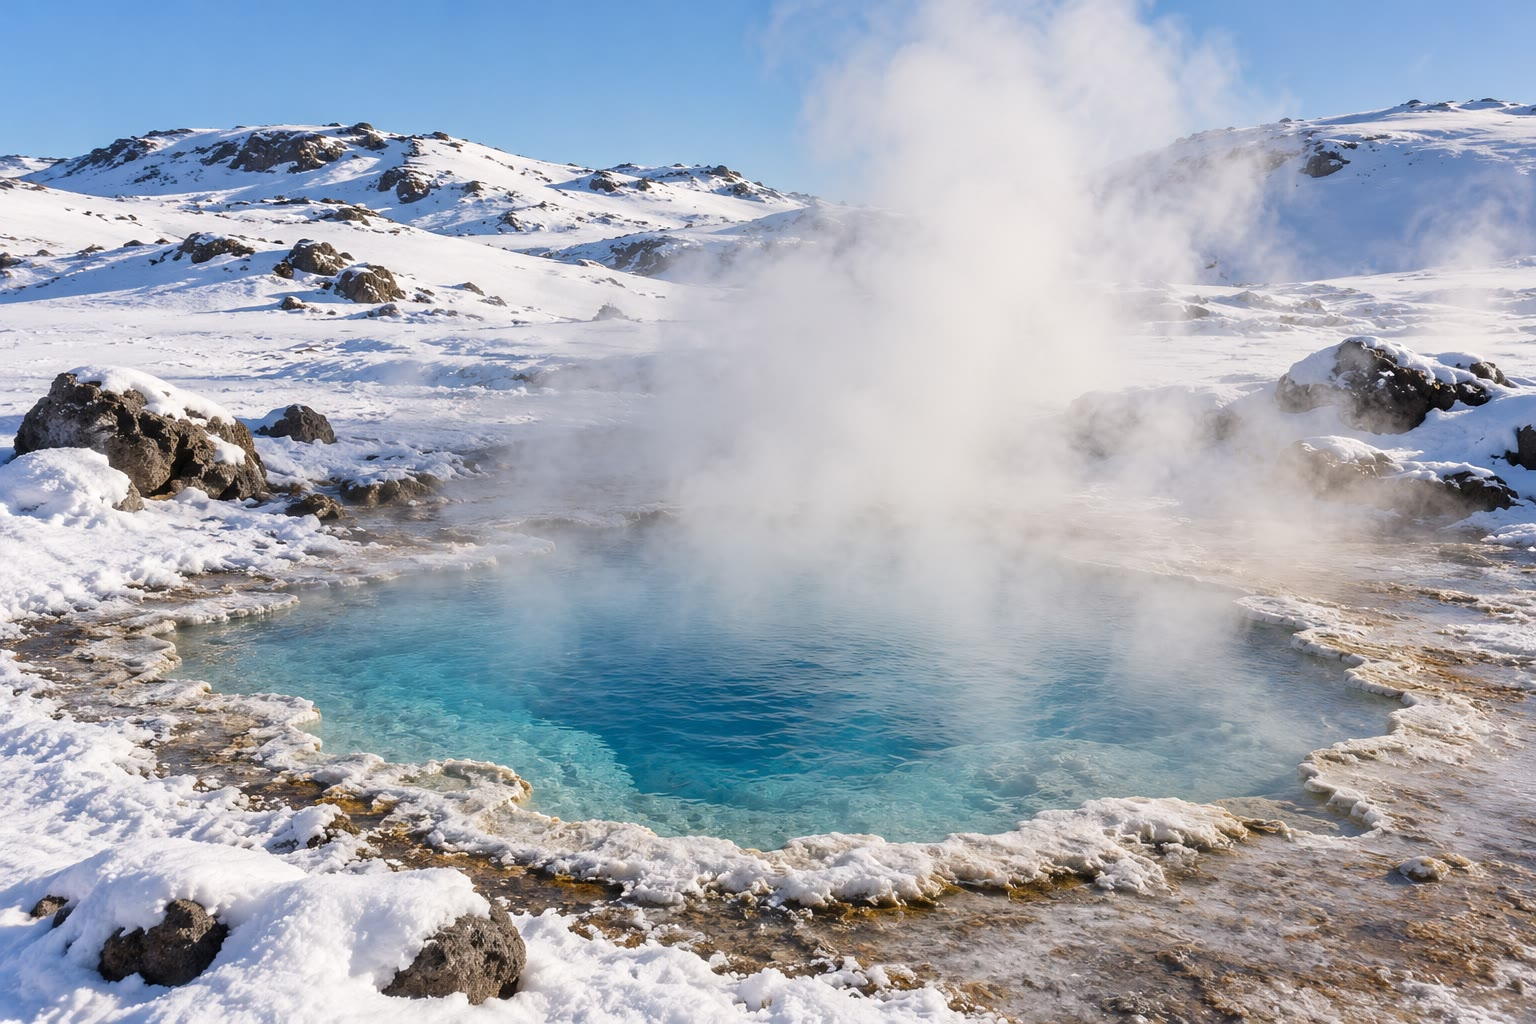
\includegraphics[width=0.6\linewidth]{images/book2/ai/g12-hot-spring-snow.jpg}

{\small A hot spring steaming in a snowy landscape: water warmed deep
underground comes back to the surface. AI-generated illustration.}
\end{omfigure}

\begin{omfigure}
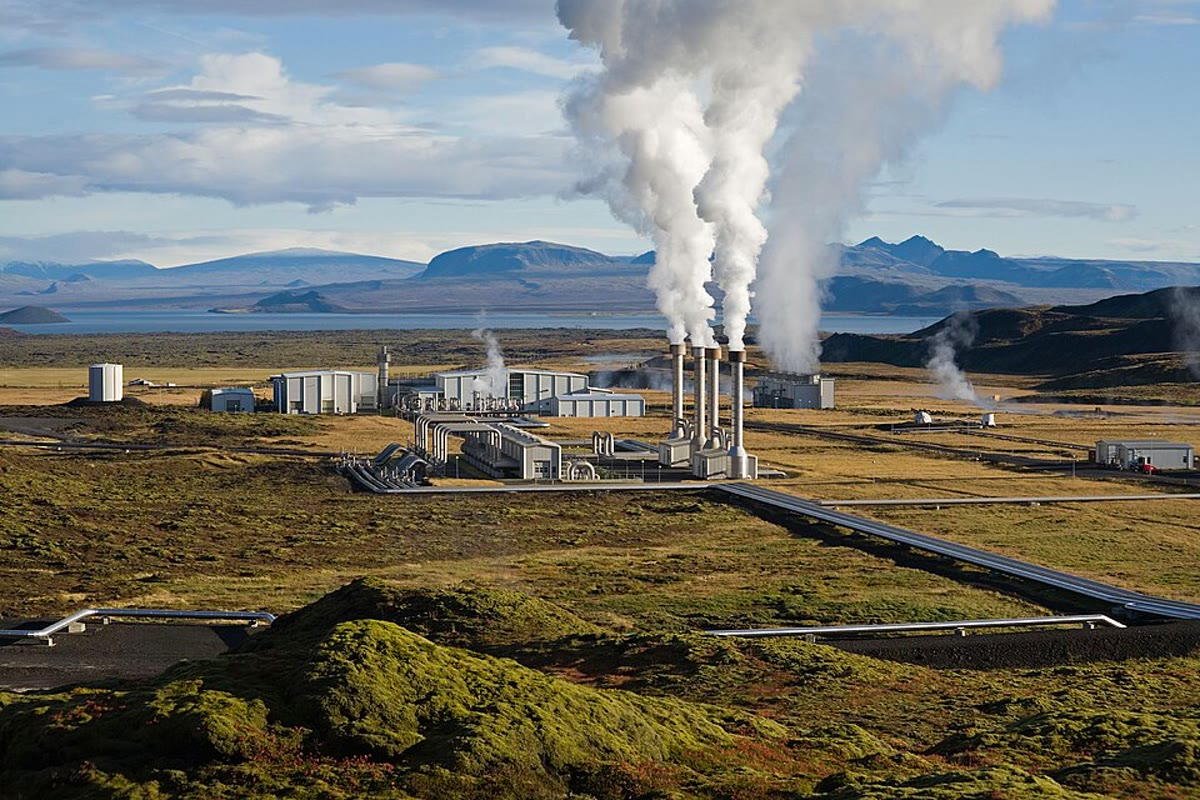
\includegraphics[width=0.66\linewidth]{images/book2/g12-nesjavellir-geothermal.jpg}

{\small The Nesjavellir geothermal power station, in the volcanic Hengill
area of Iceland: up to \qty{120}{MW} of electricity and up to
\qty{300}{MW} of heat, carried by hot water. Photograph Gretar
Ívarsson (public domain).}
\end{omfigure}
% ledger: photo:g12-nesjavellir, on:nesjavellir

A geothermal field is not inexhaustible on the scale of a human life. At The
Geysers, in California, too many wells drew on the steam, faster than the
slow \omterm{def:g12:internal-heat:heat-flow}{heat flow} and the rain could make it up: the pressure of the steam fell
to less than half its peak, and more than \qty{40}{\percent} of the
power stations' capacity was lost. Water is now injected back into the
field to slow the decline.
% ledger: cpuc:geysers

\section{Exercises}

\begin{exercise}[$\star$]\label{exo:g12:internal-heat:1}
Give the word: (a) the power leaving the interior through each square metre
of surface; (b) the heat released by the decay of radioactive atoms in a unit
volume of rock; (c) the loss of the heat stored since the Earth formed;
(d) transport of heat by the motion of the material itself; (e) the Earth's
internal heat used by people.
\end{exercise}

\begin{exercise}[$\star$]\label{exo:g12:internal-heat:2}
Convert: (1) \qty{91.6}{mW/m^2} into \unit{W/m^2}; (2) \qty{46.7}{TW} into
watts; (3) \qty{29}{\celsius} per kilometre into kelvins per metre.
\end{exercise}

\begin{exercise}[$\star$]\label{exo:g12:internal-heat:3}
Name the four isotopes that make almost all the radiogenic heat, and say
which two the KamLAND detector can see.
\end{exercise}

\begin{exercise}[$\star$]\label{exo:g12:internal-heat:4}
Using $q = 490/\sqrt{t}$, compute the \omterm{def:g12:internal-heat:heat-flow}{heat flow} through ocean floor 1, 4,
25 and 49 million years old.
\end{exercise}

\begin{exercise}[$\star$]\label{exo:g12:internal-heat:5}
Why is \omterm{def:g12:internal-heat:heat-flow}{heat flow} measured in boreholes rather than at the surface itself?
Why must one wait after drilling before measuring?
\end{exercise}

\begin{exercise}[$\star\star$]\label{exo:g12:internal-heat:6}
In the KTB borehole the rock was at about \qty{265}{\celsius} at
\qty{9.1}{km}. (1) Taking \qty{10}{\celsius} at the surface, compute the mean
gradient. (2) With a conductivity of \qty{2.72}{W/(m.K)}, what \omterm{def:g12:internal-heat:heat-flow}{heat flow}
does it give? (3) Compare with the mean of the continents.
\end{exercise}

\begin{exercise}[$\star\star$]\label{exo:g12:internal-heat:7}
The continents cover \qty{2.073e14}{m^2} with a mean \omterm{def:g12:internal-heat:heat-flow}{heat flow} of
\qty{70.9}{mW/m^2}, the oceans \qty{3.028e14}{m^2} with
\qty{105.4}{mW/m^2}. Compute the power lost by each, the total, and the share
lost through the ocean floor.
\end{exercise}

\begin{exercise}[$\star\star$]\label{exo:g12:internal-heat:8}
A layer of \omterm{def:g12:subduction-magmatism:granodiorite}{granodiorite} \qty{8}{km} thick has a heat production of
\qty{1.88}{\micro W/m^3}. (1) What \omterm{def:g12:internal-heat:heat-flow}{heat flow} does it produce at the surface?
(2) What share is that of \qty{70.9}{mW/m^2}?
\end{exercise}

\begin{exercise}[$\star\star$]\label{exo:g12:internal-heat:9}
At what age does the ocean floor lose as much heat as the mean continent,
\qty{70.9}{mW/m^2}, according to $q = 490/\sqrt{t}$?
\end{exercise}

\begin{exercise}[$\star\star$]\label{exo:g12:internal-heat:10}
How much more heat did uranium-235 release 1.4 billion years ago than
today? And potassium-40, 2.5 billion years ago?
\end{exercise}

\begin{exercise}[$\star\star$]\label{exo:g12:internal-heat:11}
Using $t \approx L^2/\kappa$ with $\kappa = \qty{1e-6}{m^2/s}$, how long
does heat take to cross by conduction (1) a lava flow \qty{10}{m} thick;
(2) a \omterm{def:g11:lithosphere-asthenosphere:lithosphere}{lithosphere} \qty{100}{km} thick; (3) the mantle? Express each result
in sensible units.
\end{exercise}

\begin{exercise}[$\star\star\star$]\label{exo:g12:internal-heat:12}
Today thorium-232 releases about \qty{10.4}{TW}, uranium-238 \qty{9.6}{TW},
potassium-40 \qty{4.0}{TW} and uranium-235 \qty{0.42}{TW}. Using the
half-lives of the figure, compute the heat of
each 3 billion years ago, the total, and the share of the two short-lived
isotopes.
\end{exercise}

\begin{exercise}[$\star\star\star$]\label{exo:g12:internal-heat:13}
The Nesjavellir power station can deliver up to \qty{300}{MW} of heat,
carried by about \qty{1640}{L} of hot water a second. With a specific heat
of \qty{4180}{J/(kg.K)} and a mass of \qty{1}{kg} per litre, by how many
degrees has this water been warmed? How large an area of average continent
loses \qty{300}{MW} of heat?
\end{exercise}

\begin{exercise}[$\star\star\star$]\label{exo:g12:internal-heat:14}
Suppose a plate takes 100 million years to go from a ridge to a trench, and a
loop of convection through the whole mantle about 200 million years. (1)
Compare these times with the 260 billion years of conduction across the
mantle. (2) Why can convection carry heat so much faster, although the
mantle moves only a few centimetres a year?
\end{exercise}

\begin{exercise}[$\star\star\star$]\label{exo:g12:internal-heat:15}
Suppose the core loses about \qty{10}{TW} of heat into the mantle across
the \omterm{def:g11:seismic-structure:core}{core--mantle boundary}, \qty{2891}{km} down. (1) What share of the
\omterm{def:g12:internal-heat:secular-cooling}{secular cooling}, \qty{22.3}{TW}, would that be? Where does the rest
come from? (2) Compute the mean \omterm{def:g12:internal-heat:heat-flow}{heat flow} across the
\omterm{def:g11:seismic-structure:core}{core--mantle boundary}, and compare it with the mean \omterm{def:g12:internal-heat:heat-flow}{heat flow} at the surface,
\qty{91.6}{mW/m^2}. (3) Why can the hot core warm the base of the mantle
although the mantle is solid?
\end{exercise}

\begin{problem}[{Weekend problem --- The Earth's heat budget}]
\label{pb:g12:internal-heat:1}
% ledger: b2dd10:continents, b2dd10:half-space, kamland11:geonu, dye12:isotopes, dye12:bse, b2vila:heat-production
% values (internal_heat.py): radiogenic 24.4 TW, secular 22.3 TW, share 0.523, K40 4.0, U235 0.42, U238 9.59
The \omterm{def:g12:internal-heat:heat-flow}{heat flow} of the Earth has been measured at more than 38\,000 places.
On average the continents lose \qty{70.9}{mW/m^2} over \qty{2.073e14}{m^2},
and the ocean floor \qty{105.4}{mW/m^2} over \qty{3.028e14}{m^2}.

\medskip
\noindent\textbf{Part I --- Heat flow and areas.}
\begin{enumerate}
  \item Check that the two areas add up to the area of a sphere of radius
        \qty{6371}{km}.
  \item What fraction of the surface is ocean floor?
  \item Why does the ocean floor lose more heat per square metre than the
        continents?
  \item Using $q = 490/\sqrt{t}$, compute the \omterm{def:g12:internal-heat:heat-flow}{heat flow} through ocean floor
        4 million years old.
  \item A borehole in granite (\qty{2.72}{W/(m.K)}) measures
        \qty{26}{\celsius} per kilometre. Is its \omterm{def:g12:internal-heat:heat-flow}{heat flow} above or below the
        continental mean?
\end{enumerate}

\medskip
\noindent\textbf{Part II --- The total.}
\begin{enumerate}[resume]
  \item Compute the power lost through the continents.
  \item Compute the power lost through the ocean floor.
  \item Add them: the total \omterm{def:g12:internal-heat:heat-flow}{heat flow} of the Earth, in terawatts.
  \item What is the mean \omterm{def:g12:internal-heat:heat-flow}{heat flow} over the whole surface?
  \item If \qty{10}{km} of granite (\qty{24.3}{mW/m^2}) lay under every
        continent, how many terawatts would it produce? Compare with the
        power lost through the continents.
\end{enumerate}

\medskip
\noindent\textbf{Part III --- Radiogenic heat.}
\begin{enumerate}[resume]
  \item KamLAND counts geoneutrinos from uranium-238 and thorium-232: together
        they release about \qty{20.0}{TW}, with \qty{3.9}{kg} of thorium in
        the Earth for each kilogram of uranium. A kilogram of uranium releases
        \qty{94.4}{\micro W} through its uranium-238 and \qty{4.10}{\micro W}
        through its uranium-235; a kilogram of thorium, \qty{26.3}{\micro W}.
        Compute the heat of uranium-238, then of uranium-235.
  \item Potassium-40 adds about \qty{4}{TW}. Compute the total radiogenic heat.
  \item Which kind of rock carries most of these elements, and where is it?
  \item Was the radiogenic heat larger or smaller 3 billion years ago? Why?
\end{enumerate}

\medskip
\noindent\textbf{Part IV --- Secular cooling.}
\begin{enumerate}[resume]
  \item What power is not supplied by radioactivity?
  \item Where does it come from?
  \item Compute the share of the \omterm{def:g12:internal-heat:heat-flow}{heat flow} supplied by \omterm{def:g12:internal-heat:secular-cooling}{secular cooling}.
  \item Models of the Earth's composition give a radiogenic heat of 11 to
        \qty{38}{TW}.
        Between which shares does the radiogenic part then lie?
  \item What carries most of this heat through the mantle?
  \item Sum up: what share of the Earth's heat loss does radioactivity supply
        today?
\end{enumerate}
\end{problem}
